\chapter{Metodologia}
\label{cap:metodologia}

Este capítulo descreve em detalhes a metodologia utilizada para reunir conceitos e conhecimentos sobre o tema deste trabalho, com o intuito de avaliar a possibilidade de prover um Controle Adaptativo através do algoritmo Dreamer, no ambiente de futebol de robôs. Na seção \ref{sec:ambiente} é explicado em detalhes como é o ambiente de futebol de robôs, detalhando pontos principais na subseção \ref{subsec:futebol_robo} e detalhando aspectos essenciais para a simulação na seção \ref{subsec:simulacao}, como dimensões, tempo de realização de tarefa e modelagem dos robôs. Na seção \ref{sec:experimentos_metricas} são abordados alguns caminhos possíveis para realização de experimentos, bem como o estabelecimento de métricas estratégicas para guiar e aprimorar a avaliação dos resultados. Por fim, na seção \ref{sec:cronograma} estabelece-se um planejamento das atividades.

%Este capítulo descreve em detalhes a metodologia proposta para o desenvolvimento do experimento e avaliação do Controle Adaptativo através do algoritmo Dreamer, no ambiente de futebol de robôs. Na Seção \ref{sec:config_ambiente} serão apresentados aspectos essenciais da configuração do ambiente escolhido, onde serão feitos os experimentos. Na Seção \ref{sec:treinamento} abordamos direções daquilo que será o processo de treinamento do agente. Na Seção \ref{sec:avaliacao} serão feitas avaliações sobre tarefas específicas que estão dentro do contexto do VSSS. Por fim, temos a Seção \ref{sec:proxs_passos} onde discutimos os próximos passos do trabalho.

% - - - - - - - - - - - - - - - - - - - - - - - - - - - - - - - - - - -
\section{Ambiente}
\label{sec:ambiente}

A categoria de futebol de robôs escolhida para este trabalho foi o IEEE Very Small Size Soccer (VSSS) \cite{regras_vss2023}. Esta categoria propõe um ambiente controlado no qual mais de um agente atua sobre ele. Assim, o algoritmo de aprendizado não saberá qual tipo de adversário irá enfrentar, até que o jogo comece, deixando este aspecto imprevisível. Já os aspectos visuais e físicos do ambiente são de baixa variabilidade, possuindo cores e tamanhos restritos e regulamentados por um manual, contendo regras e especificações sobre como deve ser o ambiente real das partidas.

%Nesta seção, descreveremos a configuração proposta do ambiente de futebol de robôs, que será utilizado para o treinamento e avaliação do agente dreamer. O intuito é que o ambiente simulado consiga proporcionar uma proximidade com as condições reais de uma partida da categoria VSSS, permitindo que o agente aprenda a tomar decisões adaptativas em cenários dinâmicos e incertos.

\subsection{Futebol de Robôs}
\label{subsec:futebol_robo}

O VSSS é uma categoria de futebol de robôs que consiste em uma partida de futebol entre duas equipes. Estas equipes, compostas por três robôs cada, devem ser autônomas. O ambiente é composto por uma câmera acima do campo, para cada equipe, e dois respectivos computadores para processar imagens, fazer os cálculos e se comunicar com os robôs da equipe, que estão em campo. Para a identificação de cada robô, dentro de cada equipe, temos o uso de tags superiores pré-definidas, previstas pelo regulamento da categoria \cite{regras_vss2023}. Para fazer a diferenciação entre equipes, a cor principal deve ser diferente, além de que nenhuma delas pode ser alaranjada, branca ou preta, já que a cor da bola é padronizada para a cor laranja e a cor do campo é preta com linhas brancas. Na Figura \ref{fig:ambiente_pequi} um diagrama contendo o fluxo do processamento de informações utilizado por uma equipe, Pequi Mecânico, da categoria.


Cada robô deve ter um tamanho máximo de 75mm x 75mm x 75mm e podem vestir uma roupagem de até 5mm de espessura. Podem pesar quanto a equipe quiser mas robôs mais pesados, mesmo tendo facilidade em ganhar na disputa de bola, tendem a gastar mais carga de bateria e terem dificuldade de alcançar velocidades maiores. Robôs mais leves podem alcançar velocidades maiores, mas tem dificuldade em ganhar disputa de bola. Durante a partida um jogador não pode, propositalmente, arrastar o oponente sem estar em disputa de bola, isso é considerado falta e a partida seria reiniciada em um ponto previsto nas regras. Estas e outras especificações podem ser encontradas nas regras oficiais da categoria IEEE Very Small Size Soccer \cite{regras_vss2023}.

    \begin{figure}[H]
     \centering
     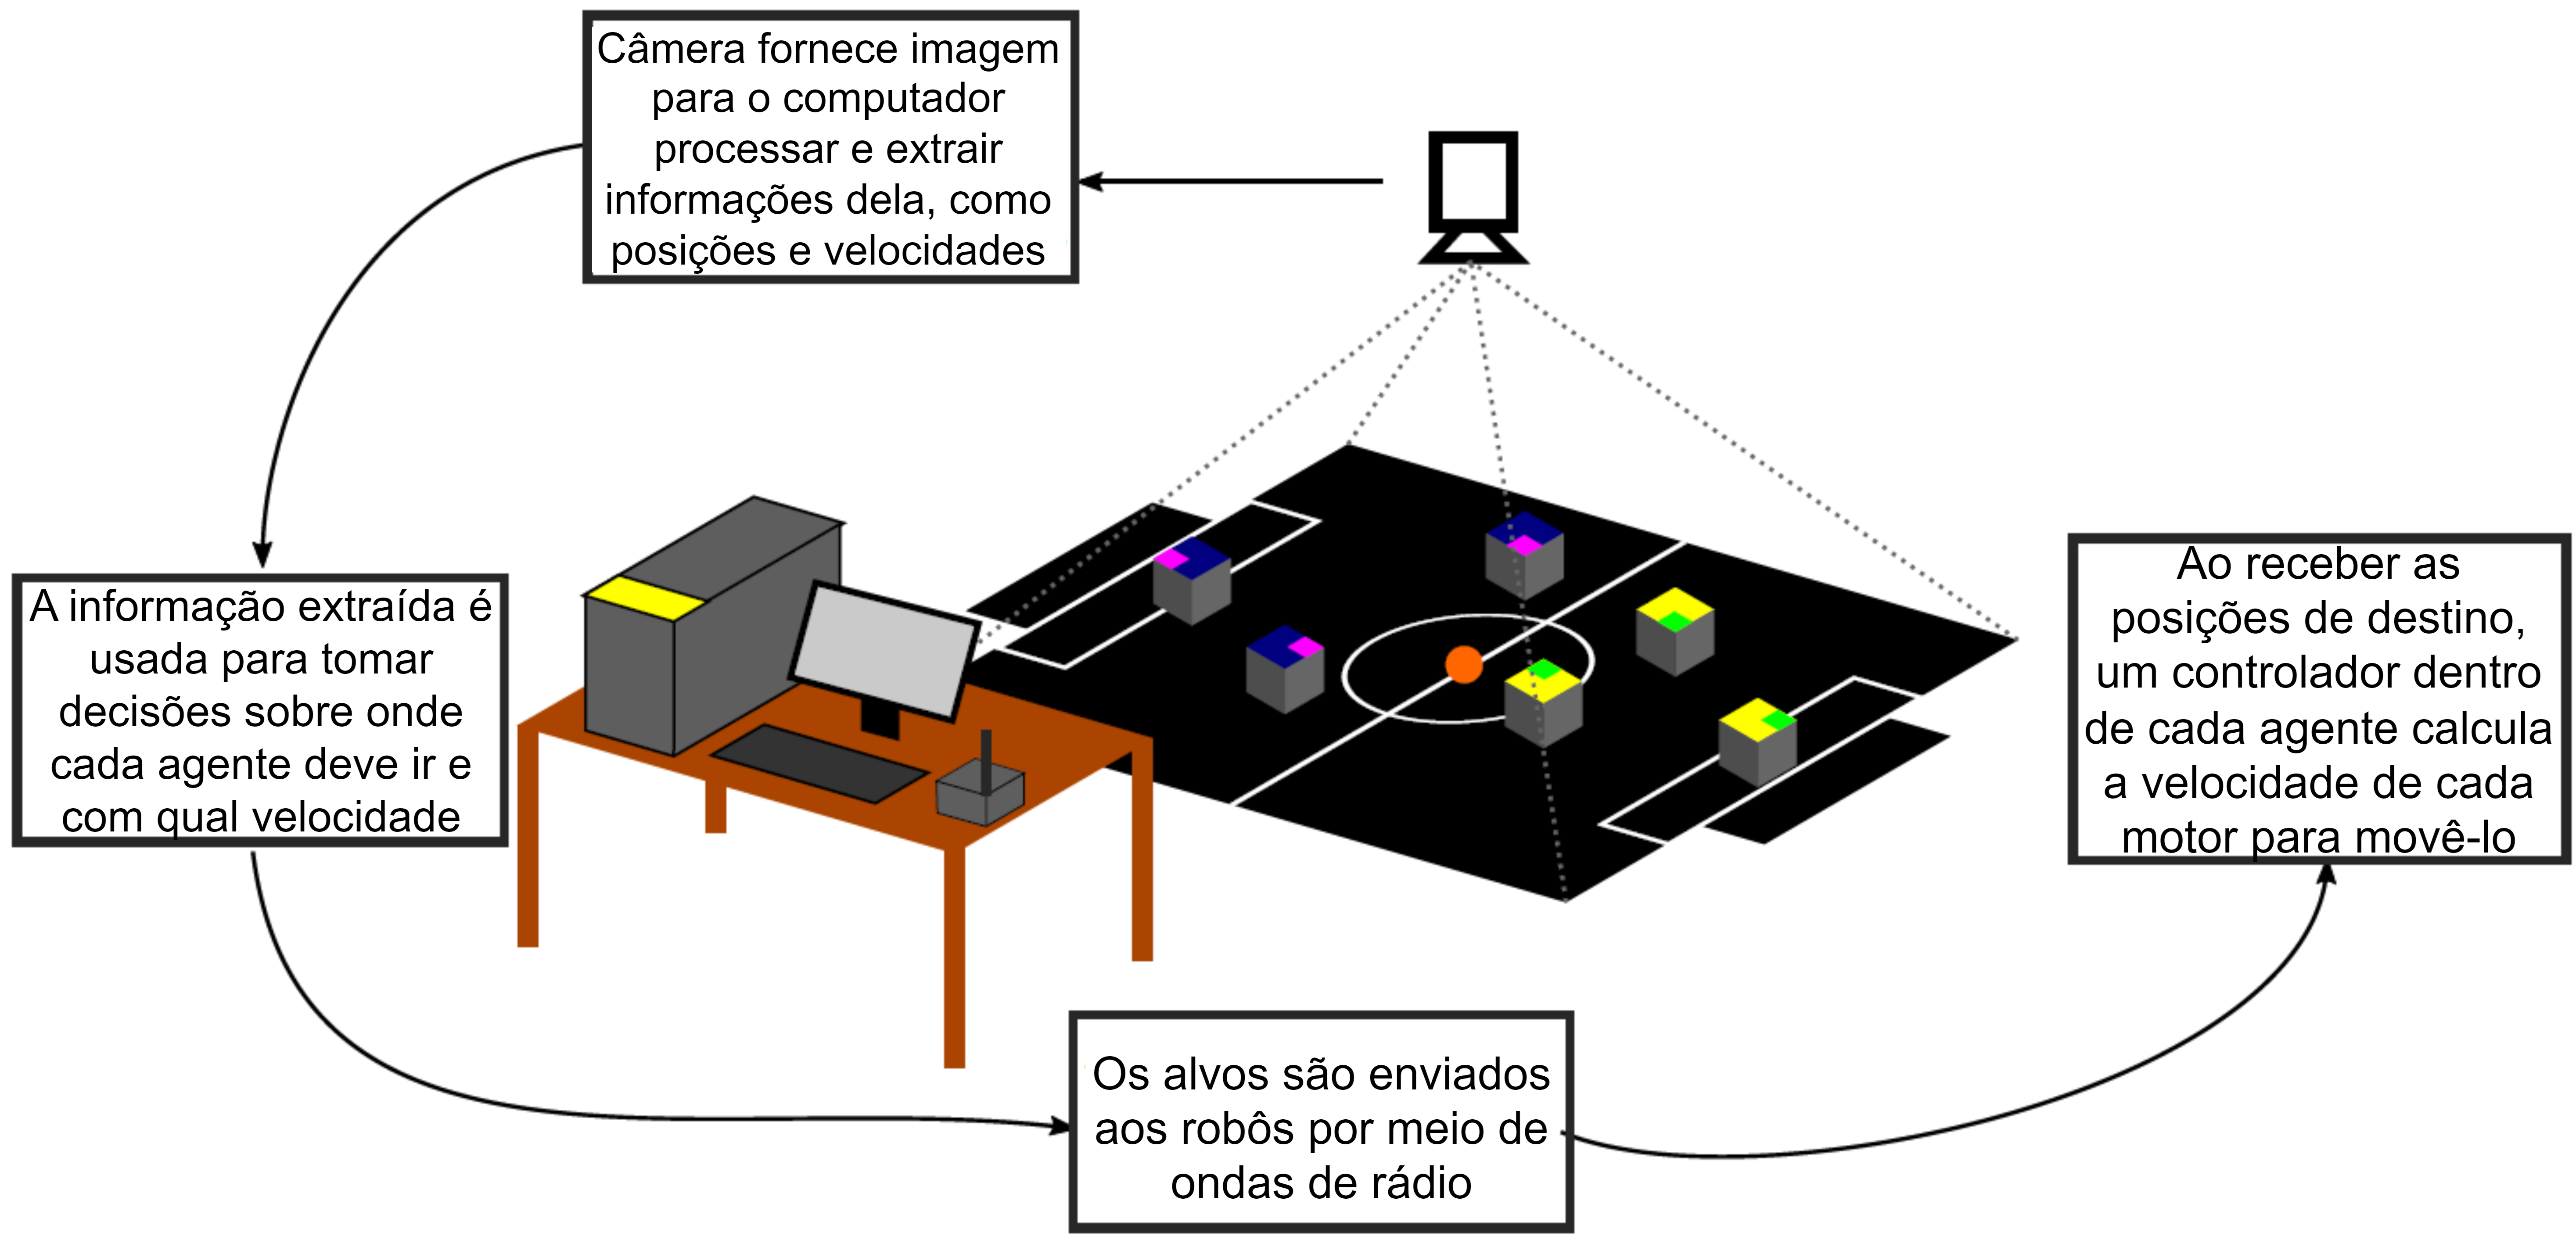
\includegraphics[width=0.85\textwidth]{./fig/ambiente_pequi.png}
    
     \caption{Diagrama do ambiente VSSS com o fluxo de informação utilizado pela equipe Pequi Mecânico \cite{bruno_brandao}.}
     \label{fig:ambiente_pequi}
    \end{figure}

%O ambiente de simulação deve ser escolhido com cautela e ponderação, já que os testes, coleta de dados e análises serão feitos por através desta simulação. Com isso, diante de algumas opções existentes dentro da categoria VSSS [FIrassim, mujoco], o ambiente que se mostrou mais adequado foi o \textit{Multi-Agent Reinforcement Learning for Robotic Soccer}\footnote{\href{https://github.com/BrunoBSM/multi-agent-soccer-self-play}{Repositório no GitHub}}, mesmo utilizado por [CITAR PAPER BRUNO].

%As características principais, que foram cruciais para a escolha, são as seguintes:

%\begin{itemize}
%    \item Baseado no simulador Multi-Joint dynamics with Contact - MuJoCo, que é gratuito.
    
%    \item Já possui modelagem do ambiente VSSS, considerando as principais variáveis.
    
 %   \item Já foi utilizado para testes em trabalho parecido [citar bruno].
    
  %  \item Projeto atualizado.
    
   % \item Contato com o desenvolvedor.
%\end{itemize}
%% - - - - - - - - - - - - - - - - - - - - - - - - - - - - - - - - - - -

\subsection{Simulação}
\label{subsec:simulacao}

Para fazer a simulação de um ambiente robótico como o VSSS é necessário um simulador de física adequado. O simulador escolhido foi o MuJoCo projetado para simulação rápida e precisa de robôs \cite{46_mujoco}, já que possui melhor desempenho que outros simuladores conhecidos \cite{44_comparacao_mujoco}, além de ter acesso gratuito e ter sido escolhido pela empresa OpenAI \cite{5_openai_gym}. Toda cena é descrita em XML e pode ser lida pelo simulador assim que é acionado.

O ambiente de simulação deve ser modelado com cautela e ponderação, já que os testes, coleta de dados e análises serão feitos por através desta simulação. Com isso, o ambiente simulado que se mostrou mais adequado foi o \textit{Multi-Agent Reinforcement Learning for Robotic Soccer}, mesmo utilizado por \cite{bruno_brandao}, que é um trabalho no mesmo contexto que esse, utilizando das mesmas métricas e sob as mesmas regras. O repositório é privado, mas o autor disponibilizou o uso para fins acadêmicos. A única mudança direta do cenário deste trabalho para aquele é que ao invés de poder ter 80mm x 80mm x 80mm, agora, deve ter no máximo 75mm x 75mm x 75mm, sendo necessário um pequeno ajuste no XML.

Na figura \ref{fig:simu_regra} observamos imagens providas pelo ambiente Multi-Agent Reinforcement Learning for Robotic Soccer em comparação com as dimensões previstas nas regras da categoria VSSS \cite{regras_vss2023}.

    \begin{figure}[H]
     \centering
     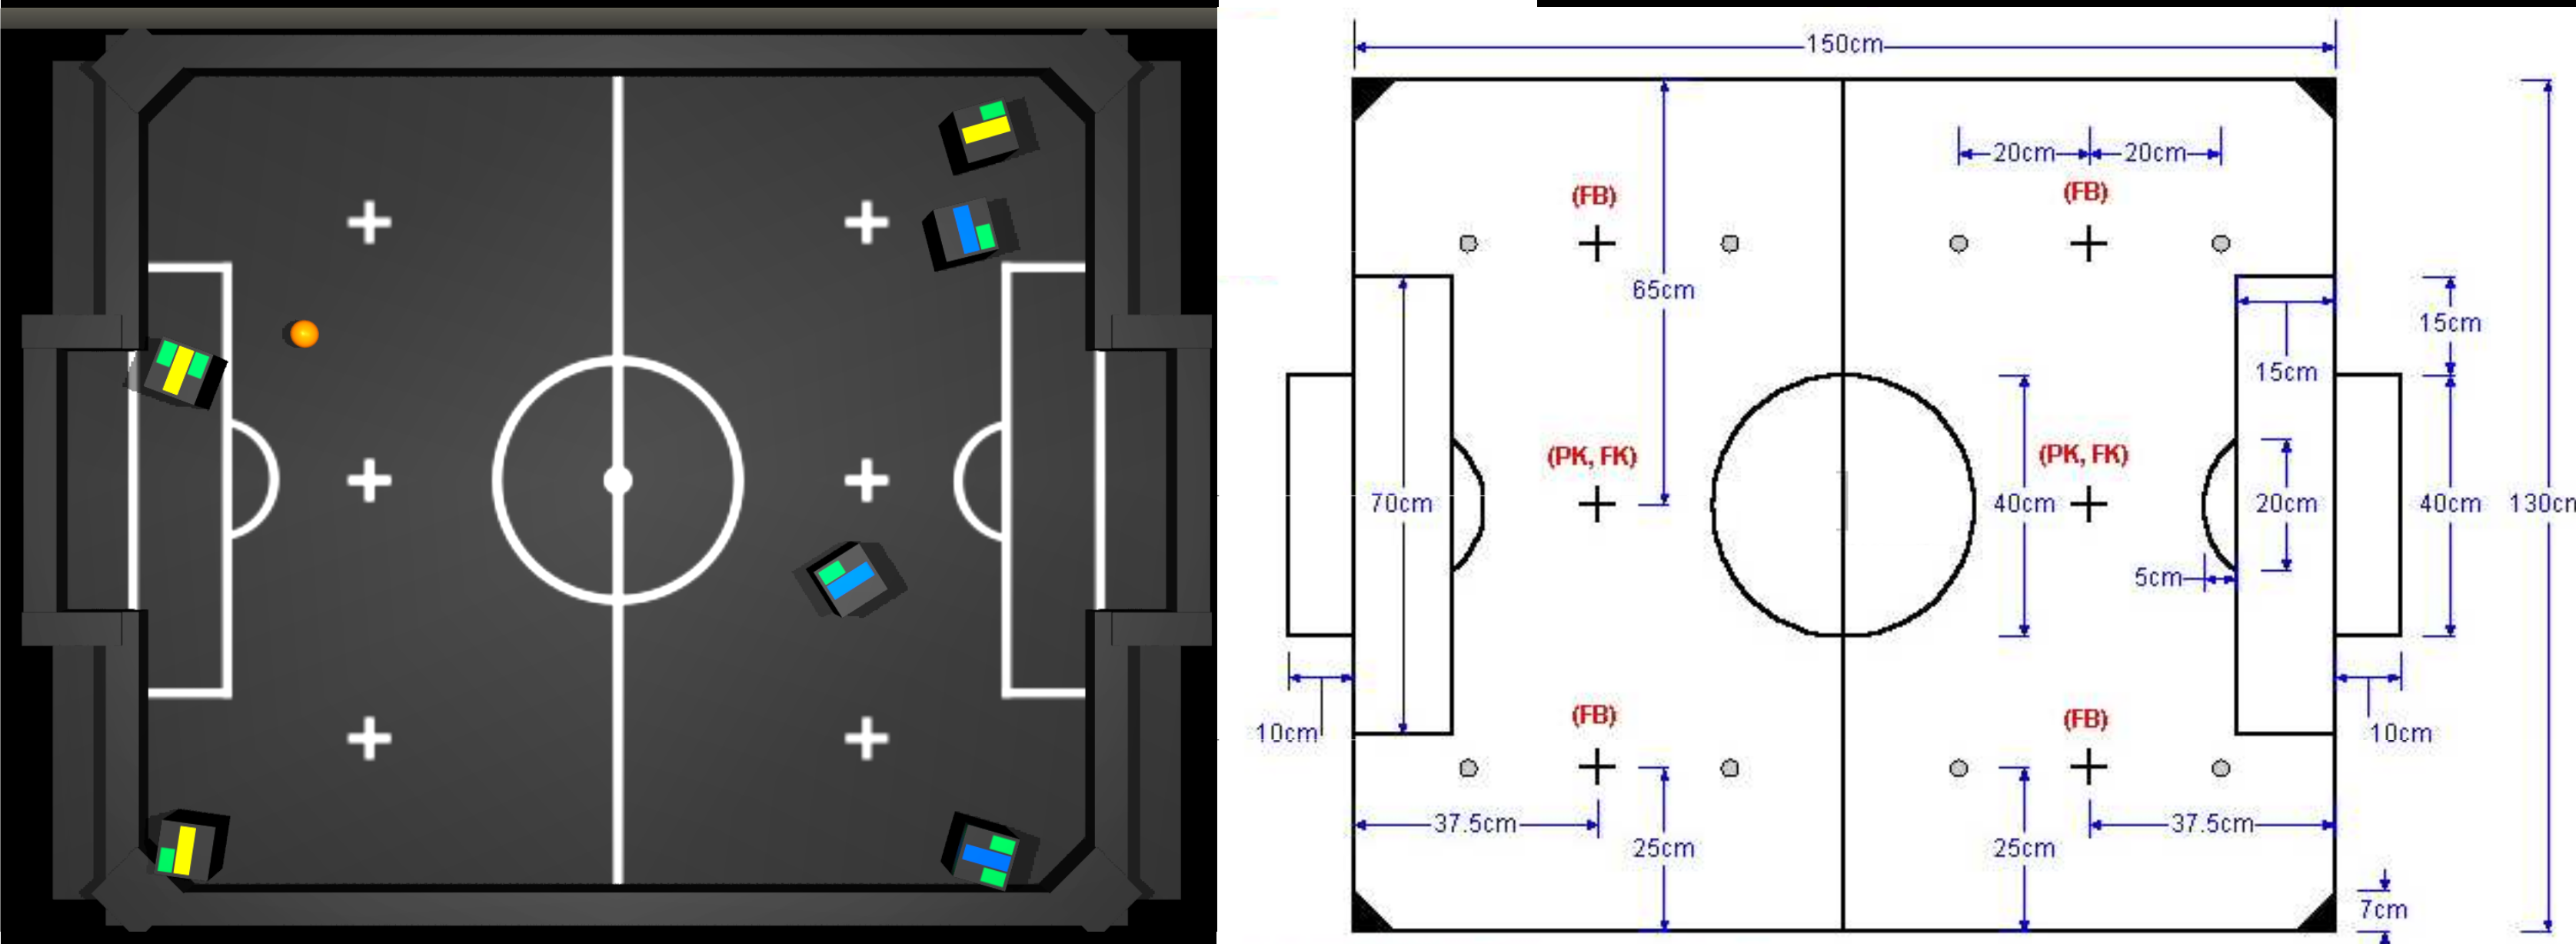
\includegraphics[width=1\textwidth]{./fig/simu_regra.png}
    
     \caption{Na esquerda imagem da simulação do ambiente Multi-Agent Reinforcement Learning for Robotic Soccer e na direita as dimensões e especificações do ambiente retirados do documento oficial das regras do VSSS \cite{regras_vss2023}.}
     \label{fig:simu_regra}
    \end{figure}


Para a modelagem dos robôs foi escolhido o modelo dos robôs reais da equipe Pequi Mecânico pelo acesso às especificações dos robôs, fácil acesso ao robô físico, facilitando qualquer eventual necessidade de comparação entre comportamentos simulados e no mundo real e prévia modelagem feita pelo ambiente Multi-Agent Reinforcement Learning for Robotic Soccer. Uma imagem da modelagem dos robôs está ilustrada no Figura \ref{fig:model_robo}.

    \begin{figure}[H]
     \centering
     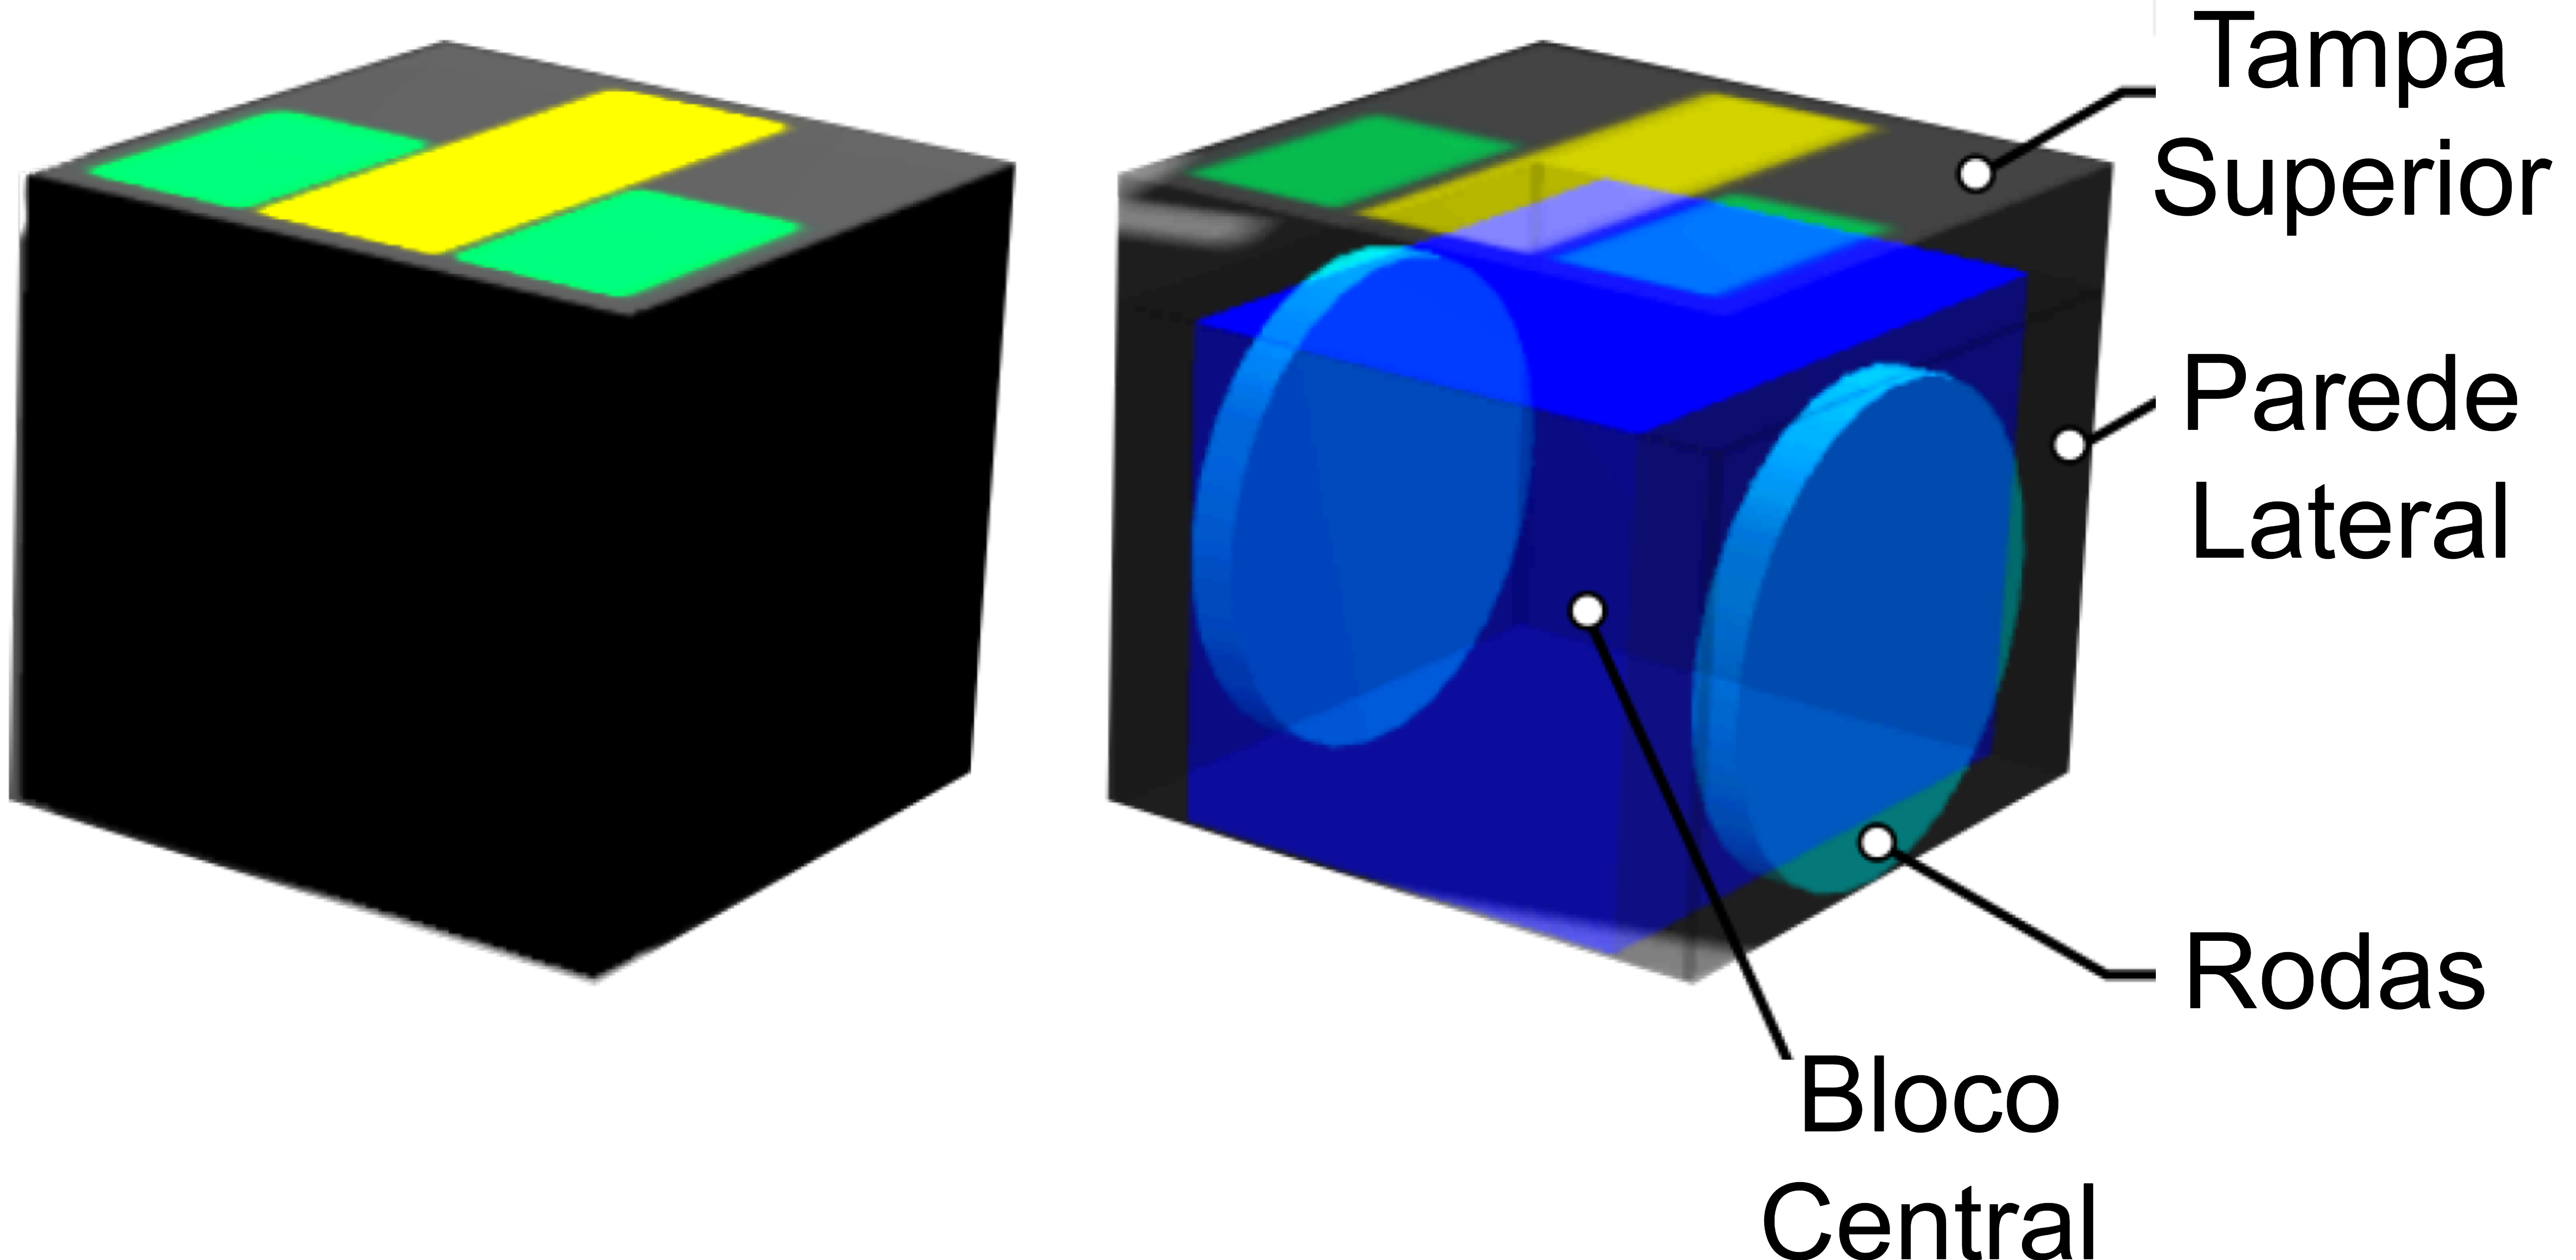
\includegraphics[width=0.8\textwidth]{./fig/model_robo.png}
    
     \caption{Exemplo da modelagem dos robôs reais da equipe Pequi Mecânico, feita pelo ambiente Multi-Agent Reinforcement Learning for Robotic Soccer.}
     \label{fig:model_robo}
    \end{figure}


\subsection*{Tempo de realização de tarefas }

Cronometrar o tempo de realização de um certa tarefa é essencial para acompanhar a evolução da velocidade do aprendizado de um agente. Com isso, o fato do ambiente  Multi-Agent Reinforcement Learning for Robotic Soccer possuir a funcionalidade de cronometrar o tempo de cada cena tornará a avaliação mais precisa para o acompanhamento da evolução do aprendizado das tarefas simples, associadas ao jogo do VSSS.

Outro ponto a ser destacado é a possibilidade de acelerar a passagem do tempo no simulador, sem comprometer a física do ambiente \cite{bruno_brandao}.


%Com base nos conteúdos desenvolvidos e nos trabalhos considerados neste trabalho, esta seção aborda os pontos e as estruturas consideradas para o treinamento do agente. O objetivo é permitir que o agente aprenda uma política adaptativa que maximize as recompensas acumuladas ao longo do tempo de treinamento.

%Abaixo estão destacados os pontos que serão abordados para executar o treinamento do agente.

%\subsubsection*{Inicialização do Agente}

%Para explorar diferentes ações e estados e evitar algumas restrições o agente será inicializado com uma política aleatória. 


%\subsubsection*{Exploração e Explotação}

%\subsubsection*{Atualização da Política}

%\subsubsection*{Curva de Aprendizado}

%\subsubsection*{Critérios de Parada}

%% - - - - - - - - - - - - - - - - - - - - - - - - - - - - - - - - - - -
\section{Tarefas}
\label{sec:tarefas}

As tarefas possuem um papel fundamental para a avaliação e validação de um solução. Como é previsto que ao final desta pesquisa deve-se obter um controle adaptativo capaz de realizar tarefas de horizonte distante, que estão inseridas em uma partida de VSSS, a definição de tarefas é essencial para o fechamento deste trabalho.

Durante uma partida de VSSS características como rapidez, movimentos estratégicos e precisão são primordiais. Com isso, este trabalho se propõe a implementar ou adaptar o algoritmo Dreamer, considerando os robôs da categoria VSSS, para a obtenção de um controle adaptativo, por meio de avaliação do desempenho nas seguintes tarefas, que estão associadas a uma partida de VSSS:

\begin{enumerate}
\item Vá para um alvo (go to target): será a tarefa mais básica, que consiste apenas em sair do ponto de partida e ir até um ponto escolhido. Neste primeiro momento não existe qualquer tipo de obstrução, apenas o agente e o campo livre.

\item \textbf{Vá para um alvo e pare em uma direção:} além da necessidade de chegar até o ponto escolhido, será necessário parar apontando para um direção definida.

\item \textbf{Vá para um alvo, com obstáculos no caminho, e pare em uma direção:} nesta tarefa será acrescentado um obstáculo fixo, deixando-a um pouco mais difícil que a tarefa anterior.

\item \textbf{Vá para um alvo com a presença de ruídos:} esta tarefa consiste em acrescentar ruídos durante a execução da tarefa anterior. O ruído poderá ser desde uma força atuando na lateral do robô, até uma deformação no corpo do robô.
\end{enumerate}

As tarefas supracitadas estão inseridas na execução de cada partida de VSSS e por isso serão chamadas de sub-tarefas, já que estas, juntamente com uma estratégia de jogo, levam a execução de uma partida completa.

É necessário ressaltar que mesmo com as tarefas selecionadas e citadas nesta seção, existe a possibilidade de outras tarefas serem consideradas futuramente, caso se mostre adequado e viável.

%% - - - - - - - - - - - - - - - - - - - - - - - - - - - - - - - - - - -
\section{Proposta de Experimentos e Métricas}
\label{sec:experimentos_metricas}


Levando em consideração os conceitos sobre RL, abordados na seção \ref{sec:RL}, o agente proposto pelo algoritmo Dreamer, abordado na seção \ref{sec:dreamer}, o contexto do futebol de robôs, representado neste trabalho pela categoria VSSS, mostrado na seção \ref{sec:ambiente} e as sub-tarefas da categoria apresentadas e detalhadas na seção \ref{sec:tarefas}, os experimentos deverão demonstrar a adaptabilidade da solução proposta a medida que as tarefas variam, aumentando o grau de dificuldade.. 

Sabe-se da mudança de dificuldade nas tarefas propostas, como mostrado na \ref{sec:tarefas}. Com isso, uma das métricas propostas será a o número de interações até a realização da tarefa, sendo que a execução das tarefas serão em sequência, começando da tarefa mais básica até a tarefa considerada mais difícil.

Existem duas formas de prosseguir com o experimento, preservando o modelo, com a tarefa aprendida anteriormente, e começando sempre do mesmo ponto, sem conhecimento prévio. Como são níveis de dificuldades diferentes constata-se que a abordagem mais adequada, até mesmo para motivos de comparação de adaptabilidade, será o experimento preservando o conhecimento adquirido para aprender a tarefa mais simples. Desta forma, ao realizar a primeira tarefa o agente iniciará sem um conhecimento prévio, mas ao começar a tarefa seguinte deverá contar com os conhecimentos adquiridos durante o processo de aprendizado da primeira tarefa e assim por diante.

Um dado importante, que será capturado, será o tempo médio para a realização de cada tarefa, que poderá ser utilizado para corroborá com a métrica de números de interações por tarefa, reforçando ou contrapondo os valores obtidos.

Outra métrica que será utilizada durante os experimentos será a o grau de proximidade com a solução perfeita, de modo que uma vez que a tarefa do agente seja ir até um ponto alvo, ao final do tempo limite, que será definido, por mais que não tenha efetivamente chegado ao alvo, existirá uma distância final entre o alvo e o agente, esta distância servirá como métrica a ser acompanhada durante os experimentos.


Os resultados presentes nas métricas observadas devem fornecer um panorama de como a solução se comporta no ambiente VSSS, realizando sub-tarefas intrínsecas a uma partida da categoria, podendo ter comparativos entre as sub-tarefas em diferentes níveis de dificuldade.

Para resumir, as questões a seguir deverão ser respondidas:

\begin{itemize}
    \item O desempenho do agente é consistente ao longo do tempo e entre diferentes tarefas?
    
    \item O agente consegue demonstrar adaptabilidade entre as diferentes tarefas?
    
    \item Qual a duração dos episódios?
    
    \item Quantas vezes o agente está obtendo êxito durante um episódio?
\end{itemize}


%Avaliação será quanto à execução de manobras:

%- Tempo de convergencia

%- Quantidade de vezes que o agente chega na recompensa 



%- Caminho até a bola

%- Chute ao Gol

%- Desvio de obstáculos

%Tudo isso de forma separada



\section{Cronograma}
\label{sec:cronograma} 

Esta pesquisa, da forma como está, compreende uma revisão bibliográfica englobando o tema principal e as técnicas chaves necessárias para desenvolver uma abordagem neste contexto. Não foram feitas implementações iniciais que pudessem ser incluídas neste trabalho. Com isso, a melhor distribuição das próximas etapas estão listadas na Tabela \ref{table:cronograma}, contemplando o período dos próximos 6 meses e prevendo implementações iniciais para prévias comparações, caso se mostre necessário. As etapas serão:

\begin{enumerate}
    \item Preparação para os experimentos: Adaptação para o contexto VSSS, ajuste de modelo, se for necessário, ajuste de função de recompensa e definição do escopo de ações \cite{11_selecao_acoes};
    
    \item Realização de experimentos de adaptabilidade: observação e coleta de dados através dos experimentos;
    
    \item Ajustes necessários;
    
    \item Análise de resultados;
    
    \item Escrita de artigo e dissertação;
    
    \item Defesa.
\end{enumerate}

\begin{table}[ht]
\centering
\begin{tabular}{|l|l|l|l|l|l|l|}
\hline
\multicolumn{1}{|c|}{Etapa} & Ago & Set & Out & Nov & Dez & Jan \\ \hline
1                           & X   &     &     &     &     &     \\ \hline
2                           &     & X   & X   & X   &     &     \\ \hline
3                           &     &     &     & X   &     &     \\ \hline
4                           &     &     &     & X   & X   &     \\ \hline
5                           &     &     &     & X   & X   & X   \\ \hline
6                           &     &     &     &     &     & X   \\ \hline
\end{tabular}
\caption{Cronograma de etapas seguintes.}
\label{table:cronograma}
\end{table}